\documentclass[11pt,a4paper,twocolumn]{article}
%\usepackage{graphicx}
%\usepackage{amsmath}
%\usepackage[latin1]{inputenc}    %% european characters can be used (Windows, old Linux)
\usepackage[T1]{fontenc}   %% get hyphenation and accented letters right
\usepackage{mathptmx}      %% use fitting times fonts also in formulas
\pagestyle{empty}                %% no page numbers!
\usepackage{geometry}            %% please don't change geometry settings!
\geometry{left=20mm, right=20mm, top=25mm, bottom=25mm, noheadfoot}

\usepackage[squaren,thinqspace]{SIunits}
\usepackage{url}
\usepackage{relsize}
\usepackage{pgfplots}
\pdfminorversion=4

%c from texinfo.tex
\def\ifmonospace{\ifdim\fontdimen3\font=0pt }

%c C plus plus
\def\C++{%
\ifmonospace%
    C++%
\else%
    C\kern-.1667em\raise.30ex\hbox{\smaller{++}}%
\fi%
\spacefactor1000 }

%c C sharp
\def\Csharp{%
\ifmonospace%
    C\#%
\else%
    C\kern-.1667em\raise.30ex\hbox{\smaller{\#}}%
\fi%
\spacefactor1000 }

\setlength{\parindent}{0pt}
\setlength{\parskip}{1ex plus 0.5ex minus 0.2ex}

\begin{document}
\thispagestyle{empty}

%\bibliography{modelica2014_ModelicaStandardTables}
%\bibliographystyle{unsrt}

\title{\textbf{Remarks on the Implementation of the Modelica Standard Tables}}
\author{Thomas Beutlich \quad Gerd Kurzbach \quad Uwe Schnabel\\
ITI GmbH\\
Schweriner Stra\ss{}e 1, 01067 Dresden, Germany\\
\{beutlich, kurzbach, schnabel\}@itisim.com}
\date{} % <--- leave date empty
\maketitle\thispagestyle{empty} %% <-- you need this for the first page

\abstract{
This article reveals some implementation details regarding the C code of the revised table interpolation blocks released with the Mod\-el\-ica Standard Library (MSL) 3.2.1. The emphasis is placed on the unique features of the CombiTimeTable which are the discontinuities by time events and the periodic extrapolation. Basic information on the interpolation by Akima splines and the available table array memory optimization options are mentioned.}

\emph{Keywords: univariate interpolation, bivariate interpolation, periodic extrapolation, time events, Akima splines}

\section{Introduction}
For many years there has been no (open source) implementation of the table interpolation blocks of the MSL. Thus, Mod\-el\-ica simulation tools either did not support the table blocks or needed to provide a custom implementation that could lead to different simulation results. One objective of releasing a backward compatible MSL 3.2.1 was to provide an open source implementation of the table blocks based on the Mod\-el\-ica external object interface. This table implementation was named \emph{Mod\-el\-ica Standard Tables} and comprises the following four blocks for univariate and bivariate interpolation
\begin{itemize}
\item Mod\-el\-ica.Blocks.Sources.CombiTimeTable,
\item Mod\-el\-ica.Blocks.Tables.CombiTable1D,
\item Mod\-el\-ica.Blocks.Tables.CombiTable1Ds and
\item Mod\-el\-ica.Blocks.Tables.CombiTable2D.
\end{itemize}

The C header and source files of the Mod\-el\-ica Standard Tables are publicly available from \url{https://svn.modelica.org/projects/Modelica/trunk/Modelica/Resources/C-Sources}. The C interface functions all start with prefix \texttt{Mod\-el\-ica\-Standard\-Tables\_}. The constructors and destructors of the external table objects have suffix \texttt{\_init} and \texttt{\_close}, respectively. If the table data is to be read from an ASCII text file or a MATLAB MAT-File, an inter\-face function with suffix \texttt{\_read} is used, i.e. file I/O is not part of the construction of the external table object. The actual interpolation functions are labeled by trailing \texttt{\_getValue} and \texttt{\_getDerValue} for the interpolation function and the interpolated derivatives, respectively.

\section{CombiTimeTable}
The block Mod\-el\-ica.Blocks.Sources.Combi\-Time\-Ta\-ble is different from standard univariate interpolation since discontinuities (by time events) and periodic ex\-trapo\-la\-tion are considered. For instance, periodic and discontinuous signals like saw-tooth or square-wave w.r.t. simulation time can be modeled in a very convenient and compact way.

\subsection{Time events}
Time events always occur at the table boundaries ($t_{min}$ and $t_{max}$) of the sample points, i.e. if interpolation switches to extrapolation.
\begin{itemize}
\item In case of linear interpolation, additional time events can be modeled by repetition of sample points in the table array. It is guaranteed that there are no time events at interval boundaries with a simple sample point only. Thus the time coordinates are not required to be strictly increasing but monotonically increasing.
\item In case of interpolation by constant segments, every interval boundary (defined by the sample points) leads to a time event, whether or not there is an actual discontinuity in the ordinate values. The time coordinates are not required to be strictly increasing but monotonically increasing. In fact, repeated sample points are not appropriate for the interpolation result.
\item Additional time events are not possible in case of interpolation with Akima splines. The time coordinates are required to be strictly increasing. (Thus care must be taken when changing the interpolation smoothness if there are repeated sample points.)
\end{itemize}

The static function \texttt{isNearlyEqual} from source file Mod\-el\-ica\-Stand\-ard\-Ta\-bles is used to tell if two double-precision floating-point numbers are (nearly) equal with relative threshold \texttt{\_EPSILON} (set to \power{10}{-10} by default).

The calculation of the next time event $t_E$ is performed in the interface function \texttt{Mod\-el\-ica\-Standard\-Tables\_\-Combi\-Time\-Table\_\-next\-Time\-Event}. For numerical reasons related to the floating-point arithmetic used, the current time~$t$ is incremented by a small fraction of the time table length, that is \texttt{\_EPSILON}$\cdot(t_{max}-t_{min})>0$. It is guaranteed that $t_E$ is greater than the current time~$t$ and that no time events are missed if the distance between two consecutive time events is greater than this numerical increment.

If no future time event is found \texttt{\_next\-Time\-Event} returns \texttt{DBL\_MAX}. Hence, care should be taken by a Mod\-el\-ica simulation tool to avoid floating-point overruns during the event handling.

For debugging purposes, time events can be traced (by means of \texttt{Mod\-el\-ica\-Format\-Message}) by defining \texttt{DEBUG\_\-TIME\_\-EVENTS} where each message line corresponds to one time event. For instance, linear interpolation and extrapolation of the 4$\times$2 example time table $[$0.25, 30; 0.5, 40; 0.5, 10; 0.75, 30$]$ results in three time events (Fig.~\ref{fig:lininex}).

\begin{figure}[!hb]
\centering
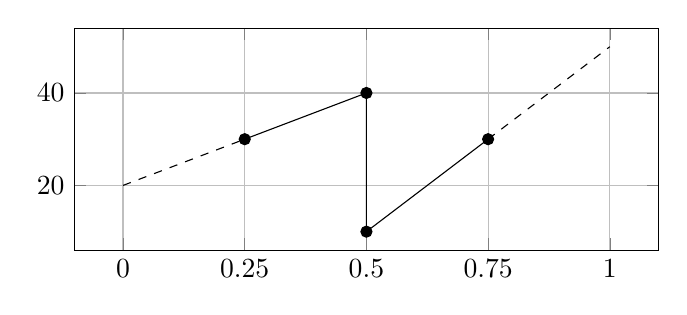
\begin{tikzpicture}
\begin{axis}[height=4.4cm, width=9cm, grid=major, enlargelimits=true, xtick={0,0.25,0.5,0.75,1}]
\addplot [mark=none] coordinates {
(0.25,30)
(0.5,40)
(0.5,10)
(0.75,30)
};
\addplot [mark=none, style=dashed] coordinates {
(0,20)
(0.25,30)
};
\addplot [mark=none, style=dashed] coordinates {
(0.75,30)
(1,50)
};
\addplot [only marks,mark=*] coordinates {
(0.25,30)
(0.5,40)
(0.5,10)
(0.75,30)
};
\end{axis}
\end{tikzpicture}
\caption{Linear interpolation of time table $[$0.25, 30; 0.5, 40; 0.5, 10; 0.75, 30$]$ results in three time events.}
\label{fig:lininex}
\end{figure}

The four messages (including the initial event) are
\begin{verbatim}
At time 0.00000: 1. time event at 0.25000
At time 0.25000: 2. time event at 0.50000
At time 0.50000: 3. time event at 0.75000
No more time events for time > 0.75000
\end{verbatim}

In order to return the correct function values at the time events (i.e. during the event iterations), the interface functions \texttt{\_getValue} and \texttt{\_getDerValue} require not only the next event time but also its pre-value as input arguments.

\subsection{Periodic extrapolation}
For tables with periodic extrapolation, the numerically stable detection of periodic time events is rather tricky. 

A first implementation was discarded as it turned out that the periodic time events were not reliably detected in all cases. The main reason is due to the IEEE 754 binary floating-point arithmetic where $t$ and $t - n\cdot T$ cannot be used simultaneously to detect the exact location of an event interval or periodic time event. Here, $t$ denotes the floating-point number (FPN) of the current time and $T=t_{max}-t_{min}$ the FPN of the period of the table. Variable $n$ is a signed integer and denotes the multiple of the period. Furthermore, let $t_E$ be the FPN of the event time (to be detected) and $t_i$ the FPN of the corresponding event interval boundary time from the table. There are FPNs such that the inequality $t \ge t_E = t_i + n\cdot T$ is true, i.e. indicates a time event, but where a simple rearrangement of the inequality to the form $t - n\cdot T \ge t_i$ does not hold. This illustrates the fact that floating-point operations cannot be used to exactly evaluate floating-point comparisons, and therefore cannot be used to reliably detect periodic time events.

% There are FPNs such that $t \ge t_E = t_i + n\cdot T$ indicates a time event, but it is $t - n\cdot T \not\ge t_i$. Hence, floating-point arithmetic must not be used to detect periodic time events.

The final implementation is based on (nonnegative) integers
\begin{itemize}
\item \texttt{nEventsPerPeriod}, the number of time events per period and
\item \texttt{event\-In\-ter\-val}, the (discrete) event interval marker.
\end{itemize}
During the very first call of function \texttt{\_next\-Time\-Event}, the number of time events per period is determined from the time coordinates of the table array. There is always a time event per period at the table boundary, thus \texttt{nEventsPerPeriod}~$\ge 1$. Furthermore, the start and end indices of each of the so-called \emph{event intervals} are determined and stored in the integer array \texttt{intervals}.

As an example, the 5$\times$2 time table $[$0, 10; 0.25, 30; 0.5, 40; 0.5, 10; 0.75, 30$]$ is considered.
\begin{itemize}
\item There are two time events per period in case of linear interpolation. The indices of the event intervals are $[$0, 2$]$ and $[$3, 4$]$, i.e. the first interval ranges from time 0 to time 0.5 and the second interval from 0.5 to 0.75 (Fig.~\ref{fig:2e}).
\begin{figure}[!htbp]
\centering
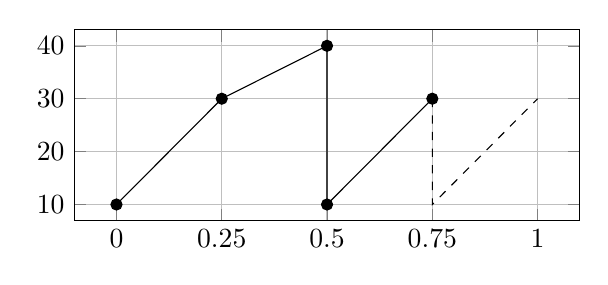
\begin{tikzpicture}
\begin{axis}[height=4cm, width=8cm, grid=major, enlargelimits=true, xtick={0,0.25,0.5,0.75,1}]
\addplot [mark=none] coordinates {
(0,10)
(0.25,30)
(0.5,40)
(0.5,10)
(0.75,30)
};
\addplot [mark=none, style=dashed] coordinates {
(0.75,30)
(0.75,10)
(1,30)
};
\addplot [only marks,mark=*] coordinates {
(0,10)
(0.25,30)
(0.5,40)
(0.5,10)
(0.75,30)
};
\end{axis}
\end{tikzpicture}
\caption{Two time events per period}
\label{fig:2e}
\end{figure}
\vspace{-5mm}
% , i.e. the first interval ranges from time 0 to time 0.25, the second interval from 0.25 to 0.5 and the third interval from 0.5 to 0.75
\item There are three time events per period in case of interpolation by constant segments. The indices of the event intervals are $[$0, 1$]$, $[$1, 2$]$ and $[$3, 4$]$. Repeated sample points are ignored since their ordinate values can never be taken by the interpolating function (Fig.~\ref{fig:3e})
\begin{figure}[!htbp]
\centering
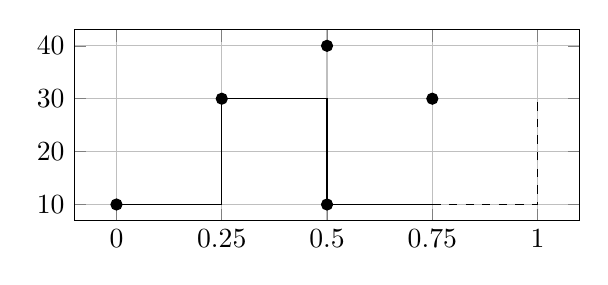
\begin{tikzpicture}
\begin{axis}[height=4cm, width=8cm, grid=major, enlargelimits=true, xtick={0,0.25,0.5,0.75,1}]
\addplot [mark=none] coordinates {
(0,10)
(0.25,10)
(0.25,30)
(0.5,30)
(0.5,10)
(0.75,10)
};
\addplot [mark=none, style=dashed] coordinates {
(0.75,10)
(1,10)
(1,30)
};
\addplot [only marks,mark=*] coordinates {
(0,10)
(0.25,30)
(0.5,40)
(0.5,10)
(0.75,30)
};
\end{axis}
\end{tikzpicture}
\caption{Three time events per period}
\label{fig:3e}
\end{figure}
\vspace{-5mm}
\end{itemize}

The event interval marker \texttt{eventInterval} uses one-based indexing. It is properly initialized once in the very first call of function \texttt{\_next\-Time\-Event} since interpolation does not need to start in the first event interval by default. Along with both integer variables and the event intervals array, the initial offset time \texttt{tOffset}~$=n\cdot T$ is determined and stored.

Each subsequent call of \texttt{\_next\-Time\-Event} now increments the event interval marker by one and resets it to~$1$ once it overruns, i.e. gets greater than the number of time events per period. This can be derived from the fact that the input variable (time) is usually increasing (w.r.t. time). Then it is known that there is exactly one time event per event interval. There is an event interval correction implemented in functions \texttt{\_getValue} and \texttt{\_getDerValue} that sets the time to be interpolated to either the left or right event interval value in case of floating-point inaccuracies. This implementation guarantees that no time events are missed and that the correct function values of the interpolating function at the event interval boundaries are returned.

\section{Interpolation by Akima splines}
Hiroshi Akima's original articles~\cite{Akima:1970:NMI:321607.321609, Akima:1974:MBI:360767.360779} were used for the implementation of the univariate and bivariate interpolation by Akima splines. His reference implementation (in FORTRAN 77) was not used. Furthermore, the FORTRAN 90 code of SOSIE~\cite{www:sosie} from Laurent Brodeau was studied for an efficient calculation of the coefficients for bivariate splines.

\subsection{Spline coefficients}
There are different possibilities to calculate and store the polynomial spline coefficients of the interpolating function.
\begin{enumerate}
\item Pre-calculate all coefficients during the initialization and store them within the external table object.
\item Calculate the coefficients whenever needed (and possibly store only the last calculated set of coefficients if used for evaluating the partial derivatives in the same simulation time step).
\item Allocate enough memory during initialization to store all coefficients, calculate them whenever needed and store them whenever calculated. The advantage is that for very large tables where only a few different data parts are accessed there will be no superfluous calculation at all and initialization time is short. The disadvantages are the high memory usage and the unpredictable execution time of a simulation time step (as it is never known if the calculated coefficients are already available).
\end{enumerate}
This implementation of the Mod\-el\-ica Standard Tables uses the first option where all required coefficients of the entire table array are calculated during initialization in function \texttt{spline1DInit} (for univariate Akima splines) and \texttt{spline2DInit} (for bivariate Akima splines).

\subsection{Differentiability}
The current univariate Akima spline interpolation always uses non-periodic table boundary conditions which may lead to a discontinuous interpolating function or derivative at the table boundaries for periodic extrapolation with the CombiTimeTable (Fig.~\ref{fig:periodic}).

\begin{figure}[!ht]
\centering
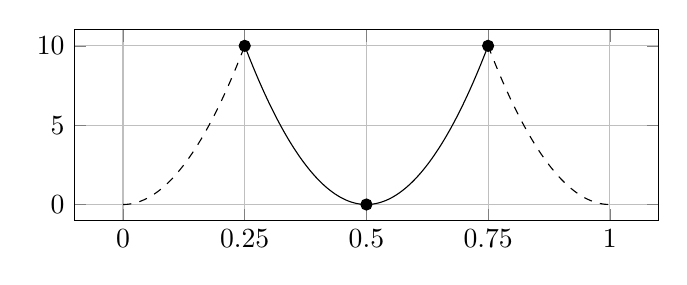
\begin{tikzpicture}
\begin{axis}[height=4cm, width=9cm, grid=major, enlargelimits=true, xtick={0,0.25,0.5,0.75,1}]
\addplot [mark=none, style=dashed] coordinates {
(0,0)
(0.005,0.00400000000000001)
(0.01,0.016)
(0.015,0.0360000000000001)
(0.02,0.0640000000000001)
(0.025,0.1)
(0.03,0.144)
(0.035,0.196)
(0.04,0.256)
(0.045,0.324000000000001)
(0.05,0.400000000000001)
(0.055,0.484000000000001)
(0.06,0.576000000000001)
(0.065,0.675999999999999)
(0.07,0.783999999999999)
(0.075,0.899999999999999)
(0.08,1.024)
(0.085,1.156)
(0.09,1.296)
(0.095,1.444)
(0.1,1.6)
(0.105,1.764)
(0.11,1.936)
(0.115,2.116)
(0.12,2.304)
(0.125,2.5)
(0.13,2.704)
(0.135,2.916)
(0.14,3.136)
(0.145,3.364)
(0.15,3.6)
(0.155,3.844)
(0.16,4.096)
(0.165,4.356)
(0.17,4.624)
(0.175,4.9)
(0.18,5.184)
(0.185,5.476)
(0.19,5.776)
(0.195,6.084)
(0.2,6.4)
(0.205,6.724)
(0.21,7.056)
(0.215,7.396)
(0.22,7.744)
(0.225,8.1)
(0.23,8.464)
(0.235,8.836)
(0.24,9.216)
(0.245,9.604)
(0.25,10)
};
\addplot [mark=none] coordinates {
(0.25,10)
(0.255,9.604)
(0.26,9.216)
(0.265,8.836)
(0.27,8.464)
(0.275,8.1)
(0.28,7.744)
(0.285,7.396)
(0.29,7.056)
(0.295,6.724)
(0.3,6.4)
(0.305,6.084)
(0.31,5.776)
(0.315,5.476)
(0.32,5.184)
(0.325,4.9)
(0.33,4.624)
(0.335,4.356)
(0.34,4.096)
(0.345,3.844)
(0.35,3.6)
(0.355,3.364)
(0.36,3.136)
(0.365,2.916)
(0.37,2.704)
(0.375,2.5)
(0.38,2.304)
(0.385,2.116)
(0.39,1.936)
(0.395,1.764)
(0.4,1.6)
(0.405,1.444)
(0.41,1.296)
(0.415,1.156)
(0.42,1.024)
(0.425,0.9)
(0.43,0.784000000000001)
(0.435,0.676)
(0.44,0.575999999999999)
(0.445,0.484)
(0.45,0.399999999999999)
(0.455,0.324)
(0.46,0.256)
(0.465,0.196)
(0.47,0.144)
(0.475,0.100000000000001)
(0.48,0.0640000000000001)
(0.485,0.0359999999999996)
(0.49,0.016)
(0.495,0.00400000000000134)
(0.5,0)
(0.505,0.00400000000000001)
(0.51,0.016)
(0.515,0.0360000000000001)
(0.52,0.0640000000000001)
(0.525,0.1)
(0.53,0.144)
(0.535,0.196)
(0.54,0.256)
(0.545,0.324000000000001)
(0.55,0.400000000000001)
(0.555,0.483999999999999)
(0.56,0.575999999999999)
(0.565,0.675999999999999)
(0.57,0.783999999999999)
(0.575,0.899999999999999)
(0.58,1.024)
(0.585,1.156)
(0.59,1.296)
(0.595,1.444)
(0.6,1.6)
(0.605,1.764)
(0.61,1.936)
(0.615,2.116)
(0.62,2.304)
(0.625,2.5)
(0.63,2.704)
(0.635,2.916)
(0.64,3.136)
(0.645,3.364)
(0.65,3.6)
(0.655,3.844)
(0.66,4.096)
(0.665,4.356)
(0.67,4.624)
(0.675,4.9)
(0.68,5.184)
(0.685,5.476)
(0.69,5.776)
(0.695,6.084)
(0.7,6.4)
(0.705,6.724)
(0.71,7.056)
(0.715,7.396)
(0.72,7.744)
(0.725,8.1)
(0.73,8.464)
(0.735,8.836)
(0.74,9.216)
(0.745,9.604)
(0.75,10)
};
\addplot [mark=none, style=dashed] coordinates {
(0.75,10)
(0.755,9.604)
(0.76,9.216)
(0.765,8.836)
(0.77,8.464)
(0.775,8.1)
(0.78,7.744)
(0.785,7.396)
(0.79,7.056)
(0.795,6.724)
(0.8,6.4)
(0.805,6.084)
(0.81,5.776)
(0.815,5.476)
(0.82,5.184)
(0.825,4.9)
(0.83,4.624)
(0.835,4.356)
(0.84,4.096)
(0.845,3.844)
(0.85,3.6)
(0.855,3.364)
(0.86,3.136)
(0.865,2.916)
(0.87,2.704)
(0.875,2.5)
(0.88,2.304)
(0.885,2.116)
(0.89,1.936)
(0.895,1.764)
(0.9,1.6)
(0.905,1.444)
(0.91,1.296)
(0.915,1.156)
(0.92,1.024)
(0.925,0.9)
(0.93,0.784000000000001)
(0.935,0.676000000000002)
(0.94,0.576000000000001)
(0.945,0.484)
(0.95,0.4)
(0.955,0.324000000000002)
(0.96,0.256)
(0.965,0.196)
(0.97,0.144)
(0.975,0.100000000000001)
(0.98,0.0640000000000001)
(0.985,0.0359999999999996)
(0.99,0.016)
(0.995,0.00400000000000134)
(1,0)
};
\addplot [only marks,mark=*] coordinates {
(0.25,10)
(0.5,0)
(0.75,10)
};
\end{axis}
\end{tikzpicture}
\caption{Periodic extrapolation of time table $[$0.25, 10; 0.5, 0; 0.75, 10$]$ by Akima splines results in a interpolating function that is not (continuously) differentiable.}
\label{fig:periodic}
\end{figure}

In all other cases it is guaranteed that the univariate or bivariate Akima spline interpolating function is continuously differentiable everywhere, especially at the table boundaries (Fig.~\ref{fig:linear}).

\begin{figure}[!h]
\centering
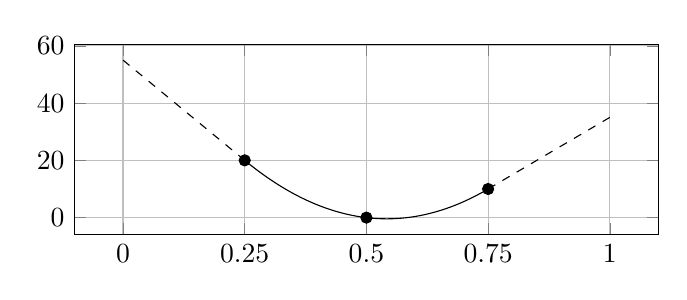
\begin{tikzpicture}
\begin{axis}[height=4cm, width=9cm, grid=major, enlargelimits=true, xtick={0,0.25,0.5,0.75,1}]
\addplot [mark=none, style=dashed] coordinates {
(0,55)
(0.25,20)
};
\addplot [mark=none] coordinates {
(0.25,20)
(0.255,19.306)
(0.26,18.624)
(0.265,17.954)
(0.27,17.296)
(0.275,16.65)
(0.28,16.016)
(0.285,15.394)
(0.29,14.784)
(0.295,14.186)
(0.3,13.6)
(0.305,13.026)
(0.31,12.464)
(0.315,11.914)
(0.32,11.376)
(0.325,10.85)
(0.33,10.336)
(0.335,9.834)
(0.34,9.344)
(0.345,8.866)
(0.35,8.4)
(0.355,7.946)
(0.36,7.504)
(0.365,7.074)
(0.37,6.656)
(0.375,6.25)
(0.38,5.856)
(0.385,5.474)
(0.39,5.104)
(0.395,4.746)
(0.4,4.4)
(0.405,4.066)
(0.41,3.744)
(0.415,3.434)
(0.42,3.136)
(0.425,2.85)
(0.43,2.576)
(0.435,2.314)
(0.44,2.064)
(0.445,1.826)
(0.45,1.6)
(0.455,1.386)
(0.46,1.184)
(0.465,0.994)
(0.47,0.816000000000003)
(0.475,0.650000000000002)
(0.48,0.495999999999999)
(0.485,0.354000000000003)
(0.49,0.224)
(0.495,0.105999999999998)
(0.5,0)
(0.505,-0.0940000000000001)
(0.51,-0.176)
(0.515,-0.246)
(0.52,-0.304)
(0.525,-0.35)
(0.53,-0.384)
(0.535,-0.406)
(0.54,-0.416)
(0.545,-0.414)
(0.55,-0.4)
(0.555,-0.374)
(0.56,-0.336000000000001)
(0.565,-0.286000000000001)
(0.57,-0.224000000000001)
(0.575,-0.150000000000001)
(0.58,-0.0640000000000009)
(0.585,0.0339999999999993)
(0.59,0.143999999999999)
(0.595,0.265999999999999)
(0.6,0.399999999999999)
(0.605,0.545999999999999)
(0.61,0.704)
(0.615,0.874)
(0.62,1.056)
(0.625,1.25)
(0.63,1.456)
(0.635,1.674)
(0.64,1.904)
(0.645,2.146)
(0.65,2.4)
(0.655,2.666)
(0.66,2.944)
(0.665,3.234)
(0.67,3.536)
(0.675,3.85)
(0.68,4.176)
(0.685,4.514)
(0.69,4.864)
(0.695,5.226)
(0.7,5.6)
(0.705,5.986)
(0.71,6.384)
(0.715,6.794)
(0.72,7.216)
(0.725,7.65)
(0.73,8.096)
(0.735,8.554)
(0.74,9.024)
(0.745,9.506)
(0.75,10)
};
\addplot [mark=none, style=dashed] coordinates {
(0.75,10)
(1,35)
};
\addplot [only marks,mark=*] coordinates {
(0.25,20)
(0.5,0)
(0.75,10)
};
\end{axis}
\end{tikzpicture}
\caption{The boundary slopes of the Akima splines are used to linearly extrapolate the one-dimensional table $[$0.25, 20; 0.5, 0; 0.75, 10$]$.}
\label{fig:linear}
\end{figure}

\section{Array memory optimizations}
Advanced array memory optimization features are implemented and explained below.

\subsection{Shared table arrays}
If multiple table objects refer to the same table array of the same file, this table array is read and stored in memory multiple times since external objects are mutually independent by default. In order to avoid superfluous file input access and to decrease the utilized memory there is a \C++ implementation of a global table array management on top of the C implementation, guarded by predefined macro \texttt{\_\_cplusplus}. The C or \C++ compilation can be toggled by compiler flag \texttt{-x c} and \texttt{-x c++} for GCC or flag \texttt{/TC} and \texttt{/TP} for Microsoft Visual C++. In the case of a \C++ compilation an additional static variable of type \texttt{TableShareMap} (using the \texttt{std::map} container from the STL) with reference counting is introduced. Write access of this global variable \texttt{tableShare} (e.g. insertion or erasure of tables) is thread-safe, i.e. guarded by a critical section (on Windows platforms) or pthread mutex (on Linux platforms) and implemented by \texttt{struct CriticalSectionHandler}.

A table array update is usually not required and therefore not implemented. Shared arrays of spline coefficients are also not implemented, i.e. each external table object always calculates and locally stores the spline coefficients it requires.

\subsection{Shallow copy of table arrays}
This optimization is only relevant if the table array is defined within the simulation model, i.e. if it is known at compile-time and not read from the file at simulation run-time. The complete table array memory that is passed from the simulation model to the constructor (the \texttt{\_init} function) of the external table object is allocated and copied (``deep copy''). This is the safe default case as nothing can be assumed about the lifetime of the table array of the simulation model. Thus the table memory is (temporarily) held twice: locally within the external table object and at the outside model. If the outside table array is known to be constant and to have a longer simulation lifetime than the external table object, the deep array copy can be avoided by defining \texttt{NO\_TABLE\_COPY}. In this case, the outside table array memory is used within the external table object (``shallow copy'' of the passed array pointer).

%\balance

\section{Conclusions}
An open source implementation of the table blocks
\begin{itemize}
\item Mod\-el\-ica.Blocks.Sources.CombiTimeTable
\item Mod\-el\-ica.Blocks.Tables.CombiTable1D
\item Mod\-el\-ica.Blocks.Tables.CombiTable1Ds
\item Mod\-el\-ica.Blocks.Tables.CombiTable2D
\end{itemize}
is available with the MSL 3.2.1 as of August 2013. The Mod\-el\-ica code is provided under Mod\-el\-ica License 2. The C/\C++ code of files Mod\-el\-ica\-Stand\-ard\-Ta\-bles and Mod\-el\-icaMatIO~\cite{www:libmatio} is provided under the new BSD license. As a result, all parts of the MSL are now available in a free implementation.

Additionally it should be mentioned that this implementation added new features to the table blocks.
\begin{itemize}
\item The new option ConstantSegments was added for the Smoothness parameter.
\item The new option NoExtrapolation was added for the Extrapolation parameter.
\item The table outputs can be differentiated once (with ex\-cep\-tion of the potentially dis\-con\-tinu\-ous Con\-stant\-Seg\-ments).
\item All MATLAB MAT-File formats are supported by an adapted library libmatio~\cite{www:libmatio} (provided by Mod\-el\-ica\-MatIO header and source file). Whereas MAT-File formats v4 and v6 are supported without additional dependencies by libmatio, the v7 format requires the zlib~\cite{www:zlib} library and compilation with preprocessor macro \texttt{HAVE\_ZLIB=1} and the v7.3 format requires the hdf5~\cite{www:hdf5} and szip~\cite{www:szip} libraries and compilation with preprocessor macro \texttt{HAVE\_HDF5=1}.
\item The support of tables provided as static C arrays in the user header file usertab.h was revised. This is relevant for real-time systems without a file system and where the table data is known at compile-time.
\end{itemize}

Last but not least, 120 test models in Mod\-el\-ica\-Test.Tables with reference results have been created.

\section{Acknowledgement}
The presented work was paid for by the Mod\-el\-ica Association.

Grateful acknowledgements go to
\begin{itemize}
\item Martin Otter for the first implementation (from 1997 till 2001) of the table interpolation blocks and for constructive discussions on the improvement of the new implementation,
\item Hans Olsson and Martin Sj\"olund for valuable advice on the improvement of the implementation,
\item Christopher C. Hulbert for sharing a MAT-File C library and providing a patch of \texttt{Mat\_Var\-Read\-Data\-Lin\-ear}~\cite{www:libmatio},
\item David Zaslavsky for initiating an interp2d library compatible with the GNU Scientific Library (GSL)~\cite{www:interp2d},
\item John C. Beatty for sharing a simple utility to concatenate multiple C source files into a single C source file~\cite{www:mergeCsource} that was used to merge header and source files of~\cite{www:libmatio} to single files Mod\-el\-ica\-MatIO.h and Mod\-el\-ica\-MatIO.c,
\item Laurent Brodeau for sharing a bivariate Akima algorithm (in FORTRAN 90)~\cite{www:sosie}.
\end{itemize}

\begin{thebibliography}{00}
\addcontentsline{toc}{chapter}{References}

\bibitem{Akima:1970:NMI:321607.321609}
Hiroshi Akima.
\newblock A new method of interpolation and smooth curve fitting based on local
  procedures.
\newblock {\em J. ACM}, 17(4):589--602, October 1970.

\bibitem{Akima:1974:MBI:360767.360779}
Hiroshi Akima.
\newblock A method of bivariate interpolation and smooth surface fitting based
  on local procedures.
\newblock {\em Commun. ACM}, 17(1):18--20, January 1974.

\bibitem{www:sosie}
Laurent Brodeau.
\newblock {SOSIE} is {O}nly a {S}urface {I}nterpolation {E}nvironment.
\newblock \url{http://sosie.sourceforge.net}.

\bibitem{www:libmatio}
Christopher~C. Hulbert.
\newblock {MAT} {F}ile {I}/{O} library version 1.5.2.
\newblock \url{http://matio.sourceforge.net}.

\bibitem{www:zlib}
Jean-Loup Gailly and Mark Adler.
\newblock {A} general purpose compression library version 1.2.8.
\newblock \url{http://zlib.net}.

\bibitem{www:hdf5}
The~HDF Group.
\newblock {H}ierarchical data format version 5.
\newblock \url{http://www.hdfgroup.org/HDF5}.

\bibitem{www:szip}
The~HDF Group.
\newblock {S}cience data lossless compression library version 2.1.
\newblock \url{http://www.hdfgroup.org/doc_resource/SZIP}.

\bibitem{www:interp2d}
David Zaslavsky.
\newblock {A} 2{D} interpolation library compatible with {GSL}.
\newblock \url{https://github.com/diazona/interp2d}.

\bibitem{www:mergeCsource}
John~C. Beatty.
\newblock {A} very simple inclusion processor.
\newblock \url{https://www.student.cs.uwaterloo.ca/~cs241/cLibs/mergeCsource}. 

\end{thebibliography}

\end{document}
